\subsection{A large-network spatial explanation}\label{sec:anaheim}
The public Anaheim network has 416 nodes, 914 directed links and 1,406 positive OD demands \citep{tnfrc2024transportation}. Six largest demands change jointly from 0.8 to 1.2 times their published values; other demands remain fixed with endogenous route choices. Ten fixed free-flow shortest paths per OD exclude other zone centroids as intermediate nodes (first through node 39). This calculation uses the existing 41-state attribution columns.
To obtain interpretable region locations without requiring coordinates, define free-flow progress $p(v)=[d_s(v)-d_t(v)+d_s(t)]/[2d_s(t)]$, using shortest distances in the underlying undirected network with the smaller free-flow time on parallel roads --- a network-distance indicator used for ordering the family, not a behavioural travel progress (assignment paths additionally exclude other zone centroids, the progress metric does not). The origin has progress zero and destination progress one. Group tied levels, retain prefixes with two connected induced sides that separate the OD, and orient every region toward the origin. This distance-based family depends on the network and query, before inspecting any attribution. It is a prescribed family, not all connected regions, and it is single-direction: the nested prefixes are totally ordered by progress, so no direction grouping is needed here.

The case asks one transport question: for a prespecified demand change,
where along the origin--destination direction does the signed
crossing-cost response change markedly, and does the variation come
mainly from the study traffic's congestion adjustment or from
background rerouting? Figure~\ref{fig:anaheimprofile} displays the
query with the largest early--late attribution difference, $(25,2)$,
chosen to illustrate the method at its richest variation; the
aggregate statistics come from all six queries
(Table~\ref{tab:anaheimsegments}). The figure shows the boundary
attribution as a function of progress over the complete family with its
reported four-segment summary, and the four-part mechanism
decomposition along the same axis. The profiles of the remaining five
queries stay positive with family ranges spanning roughly one to one
and a half orders of magnitude (largest-to-smallest attribution ratios
12.5--36.9); the complete per-query numbers --- system contributions,
unrestricted and family ranges, region counts and the attributions of
the three prespecified positions --- are collected in
Appendix~\ref{app:anaheimsettings} (Table~\ref{tab:anaheim}), with the
early--late mechanism differences in Table~\ref{tab:anaheimmechanism}.
\begin{figure}[t]\centering
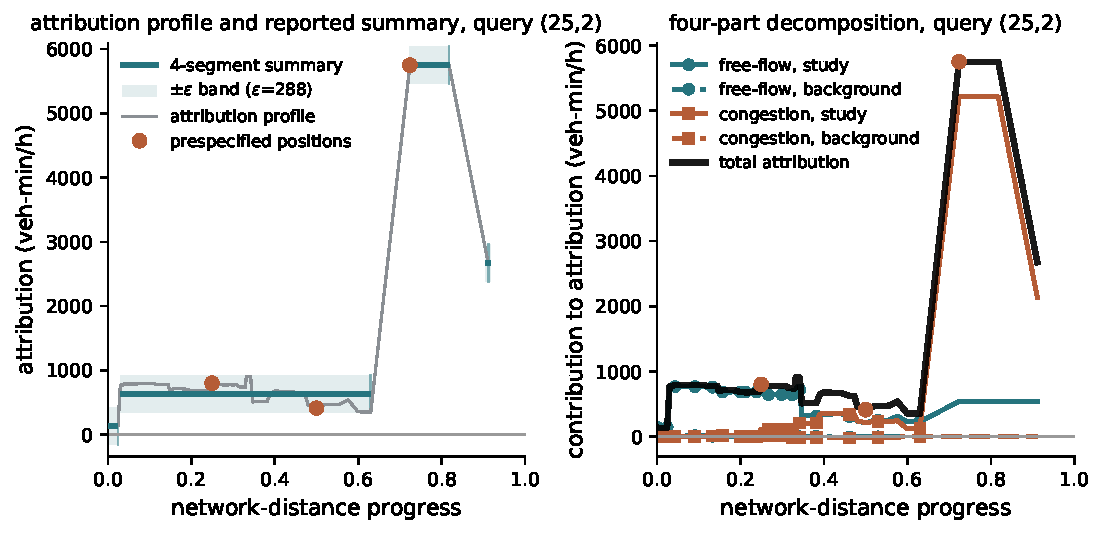
\includegraphics[width=0.99\linewidth]{../figures/fig_v108_anaheim_profile.pdf}
\caption{Anaheim boundary-attribution profile for query $(25,2)$ over
the distance-based family, with its reported summary. Left: attribution
versus free-flow progress along the OD direction (grey curve); the
four-segment minimum summary at the family tolerance (teal step curve
with $\pm\epsilon$ band, $\epsilon=287.6$); ochre dots mark the three
prespecified positions. Right: the four-part mechanism decomposition
(teal: free-flow weights, ochre: congestion weights; solid: study
response, dashed: background); the grey curve is the total
attribution.}\label{fig:anaheimprofile}
\end{figure}

\paragraph{Where the attribution changes.}
The Anaheim TNTP files ship no node coordinates, so the location layer
is reported through the crossing links of each boundary rather than a
map. Table~\ref{tab:anaheimcrossing} lists, at the three prespecified
positions and at the plateau boundary, the region size, the crossing
links, and the principal signed attribution contributions (a positive
entry adds to the attribution of the region containing the origin). The
three positions sit at very different network locations: the early
boundary crosses 34 links with two dominant contributions; the middle
boundary crosses only four links; and the high plateau corresponds to
the cut that isolates the destination neighbourhood, where the entire
attribution crosses on the single link $63\!\to\!62$.
\begin{table}[t]\centering\footnotesize
\caption{Location layer of the $(25,2)$ case: the boundary at each
reported position, its crossing links, and the principal signed
attribution contributions (vehicle-minutes per hour; positive entries
add to the origin-side attribution). Regions contain the origin; the two
plateau endpoints share the attribution $5{,}751.2$ on link
$63\!\to\!62$, while their second crossing link differs ($87\!\to\!86$
at the start, $2\!\to\!87$ at the end, contributing $-0.0$ at
both).}\label{tab:anaheimcrossing}
\setlength{\tabcolsep}{4pt}
\begin{tabular*}{\tblwidth}{@{\extracolsep{\fill}}lrrrl}
\toprule
Position & Region & Crossing & Principal links & Attribution\\
(progress) & (nodes) & links & (from$\to$to, contribution) &\\
\midrule
Early $0.250$ & 231 & 34 & $269\!\to\!261$ $+550.5$;\ $271\!\to\!192$ $+163.9$ & $801.5$\\
Middle $0.500$ & 405 & 4 & $191\!\to\!190$ $+297.0$;\ $66\!\to\!65$ $+105.4$ & $412.0$\\
Plateau $0.724$--$0.818$ & 413--414 & 2 & $63\!\to\!62$ $+5{,}751.2$;\ ($87\!\to\!86$/$2\!\to\!87$ $-0.0$) & $5{,}751.2$\\
Destination $0.911$ & 415 & 2 & $62\!\to\!2$ $+2{,}673.1$;\ ($2\!\to\!87$ $-0.0$) & $2{,}673.1$\\
\bottomrule\end{tabular*}\end{table}

\paragraph{Which traffic generates the change.}
The decomposition panel locates the mechanism. At the early position
the attribution is dominated by the free-flow study response ($669.3$
of the total $801.5$, congestion study $111.5$, background below $11$);
at the middle position the two study terms are comparable ($211.5$
free-flow against $212.6$ congestion of the total $412.0$, background
below $11$); at the late position the congestion study term reaches
$5213.7$ while both background terms are below $0.1$ in absolute value:
the rise is congestion adjustment of the study traffic itself on the
destination-side crossing link, not background rerouting. The
decomposition is additive at a common equilibrium state and attributes
the variation to the corresponding response--weight components; the
summary then states, with its error bound, where that variation
changes.

\paragraph{The reported summary.}
Table~\ref{tab:anaheimsegmentsfull} reports the complete four-segment
summary for this query: each segment's position range, the number of
boundary values it summarizes, its representative value, and the actual
worst error within the segment. An origin-side segment covers the six
boundaries nearest the origin at representative value $134.3$ (worst
error $2.5$); one long corridor segment summarizes the 75 boundaries
from progress $0.03$ to $0.63$ at $630.2$ (worst error $279.2$); the
congestion plateau is one segment at $5{,}751.2$ spanning progress
$0.724$--$0.818$; and the destination-side boundary at progress
$0.911$ is reported exactly. Every attribution lies within
$\epsilon=287.6$ of its segment value, the tolerance being $5\%$ of
the family maximum $5{,}751.2$; the reader absorbs four numbers in
place of $84$.
\begin{table}[t]\centering\footnotesize
\caption{The complete reported summary for query $(25,2)$ at the
family tolerance ($\epsilon=287.6$; vehicle-minutes per hour). Each row
is one segment: its progress range, the number of summarized boundary
values, the representative value, and the actual worst error within the
segment (at most $\epsilon$ by construction).}\label{tab:anaheimsegmentsfull}
\setlength{\tabcolsep}{5pt}
\begin{tabular*}{\tblwidth}{@{\extracolsep{\fill}}lrrrr}
\toprule
Segment & Progress range & Boundaries & Representative & Worst error\\
\midrule
1 (origin side) & $0.000$--$0.024$ & 6 & $134.3$ & $2.5$\\
2 (corridor) & $0.030$--$0.630$ & 75 & $630.2$ & $279.2$\\
3 (plateau) & $0.724$--$0.818$ & 2 & $5{,}751.2$ & $0.0$\\
4 (destination) & $0.911$ & 1 & $2{,}673.1$ & $0.0$\\
\bottomrule\end{tabular*}\end{table}
Across the six study queries the compression is uniform:
Table~\ref{tab:anaheimsegments} shows 83--211 boundary values reducing
to 4--14 segments under the compact tolerance and 6--17 under the
balanced tolerance, with every boundary value within its stated
tolerance by construction; the summary never changes an original
attribution --- it is the same computed profile at its coarsest
resolution that meets the tolerance. The balanced rule controls the
relative error at small attributions (median worst small-value relative
error $54.9\%$ under the compact rule against $27.8\%$ under the
balanced rule) at a modest segment cost (median 10 against 12).
Aggregation timings and the original construction costs appear in
Appendix~\ref{supp:timing}; the full tolerance sensitivity, including
the mixed absolute--relative rule of Section~\ref{sec:segments},
appears in Appendix~\ref{supp:tolerance}.
\begin{table}[t]\centering\footnotesize
\caption{Reported minimum-segment summaries on Anaheim under the two
tolerance settings of Section~\ref{sec:segments}
(Proposition~\ref{prop:segmented}): compact ($5\%$ of the largest
attribution magnitude per query) and balanced ($1\%$ absolute floor
plus $10\%$ relative). Worst rel.\ small: worst relative error at
small-magnitude positions (magnitude below one tenth of the family
maximum). Every boundary value in a segment lies
within its tolerance of the representative value; the complete $(25,2)$
compact segmentation appears in
Table~\ref{tab:anaheimsegmentsfull}.}\label{tab:anaheimsegments}
\setlength{\tabcolsep}{4pt}
\begin{tabular*}{\tblwidth}{@{\extracolsep{\fill}}lrcccc}
\toprule
 & & \multicolumn{2}{c}{Compact ($5\%$)} & \multicolumn{2}{c}{Balanced ($1\%{+}10\%$)}\\
\cmidrule(lr){3-4}\cmidrule(lr){5-6}
Query & Regions & Segments & Worst rel.\ small (\%) & Segments & Worst rel.\ small (\%)\\
\midrule
$(4,2)$ & 211 & 12 & 94.1 & 13 & 31.9\\
$(1,2)$ & 83 & 8 & 53.6 & 11 & 45.0\\
$(2,4)$ & 211 & 14 & 38.3 & 17 & 3.2\\
$(3,2)$ & 157 & 8 & 56.3 & 11 & 31.4\\
$(25,4)$ & 164 & 13 & 0.0 & 13 & 0.0\\
$(25,2)$ & 84 & 4 & 79.5 & 6 & 24.2\\
\bottomrule\end{tabular*}\end{table}
